% Dokumentace projektu GAL 2014
% Vendula Poncová, xponco00
% Alena Chernikava, xcerni07

\documentclass[a4paper, 11pt, titlepage, final]{article}[3. prosinec 2011]

\newcommand{\uv}[1]{\quotedblbase #1\textquotedblleft}
\newcommand{\mensi}{$<$}
\newcommand{\vetsi}{$>$}

\usepackage[left=2.5cm,text={16cm, 25cm},top=2cm]{geometry}
\usepackage[czech]{babel}
\usepackage[utf8]{inputenc}
\usepackage[IL2]{fontenc}
\usepackage[dvipdf]{graphicx}
\usepackage{color}

\newcommand{\url}[1]{\textit{#1}}
\begin{document}

%%%%%%%%%%%%%%%%%%%%%%%%%%%%%%%%%%%%%%%%%%%%%%%%%%%%%%%%%%%%%%%%%%%%%%%%%
% titulni strana - DON'T TOUCH! MAGIC!

\begin{titlepage}
\begin{center}

\textsc{
\Large Fakulta informačních technologií 
\medskip\\
Vysoké učení technické v~Brně}

\vspace{\stretch{0.190}}

{\parbox{5cm}{\centering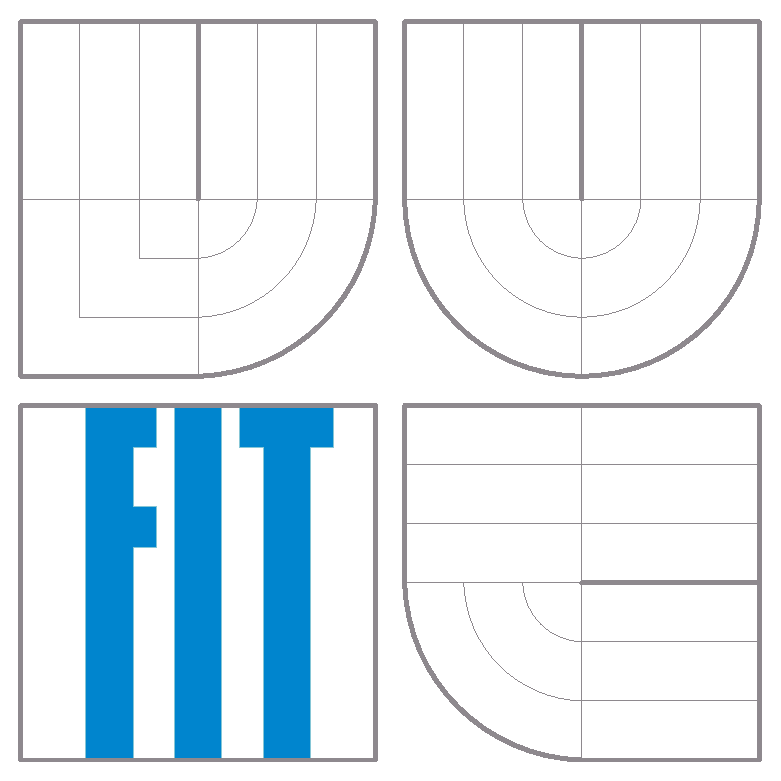
\includegraphics[height=5cm]{img/logo.eps}}}

\vspace{\stretch{0.190}}

{\LARGE Dokumentace projektu do předmětu GAL} \medskip \\
{\Large Paralelizace Egerváryho algoritmu} 


\vspace{\stretch{0.618}}

\end{center}

{\large
Tým 33

Vendula Poncová (\texttt{xponco00})

Alena Chernikava (\texttt{xcerni07})
} \hfill {\large\today}

\end{titlepage}

%%%%%%%%%%%%%%%%%%%%%%%%%%%%%%%%%%%%%%%%%%%%%%%%%%%%%%%%%%%%%%%%%%%%%%%%%
% text dokumentace

\pagenumbering{arabic}
\setcounter{page}{1}

%%%%%%%%%%%%%%%%%%%%%%%%%%%%%%%%%%%%%%%%%%%%%%%%%%%%%%%%%%%%%%%%%%%%%%%%%
\section{Úvod}

%%%%%%%%%%%%%%%%%%%%%%%%%%%%%%%%%%%%%%%%%%%%%%%%%%%%%%%%%%%%%%%%%%%%%%%%%
\section{Egerváryho algoritmus}


\begin{figure}[ht]
  \centering
  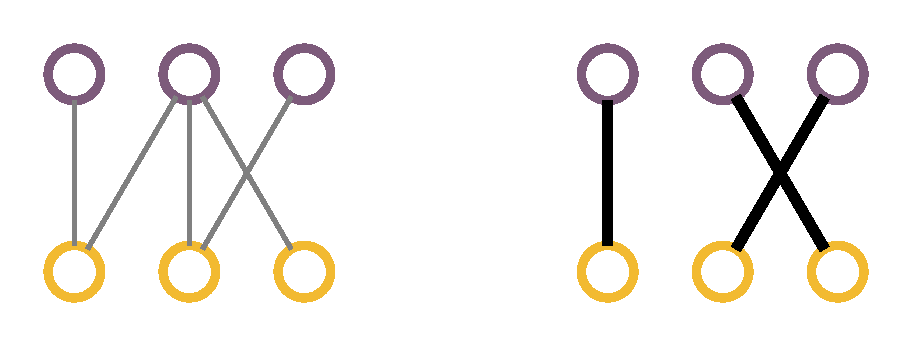
\includegraphics[scale=0.5]{img/bipartite.eps}
  \caption{Bipartitní graf a maximální párování v tomto grafu.}
  \label{imgBipartite}
\end{figure}

\begin{figure}[ht]
  \centering
  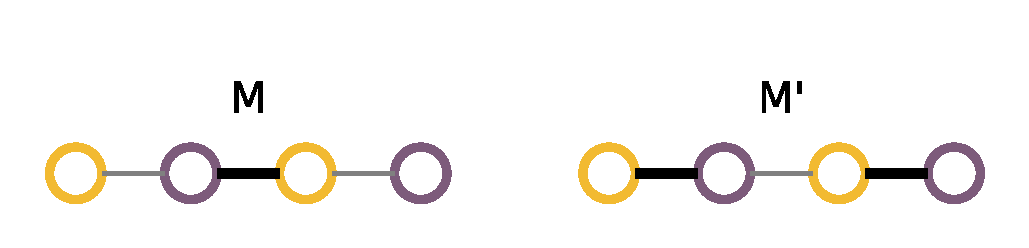
\includegraphics[scale=0.5]{img/mpath.eps}
  \caption{M-rozšiřující cesta a nové párování M'.}
  \label{imgPath}
\end{figure}

\begin{figure}[ht]
  \centering
  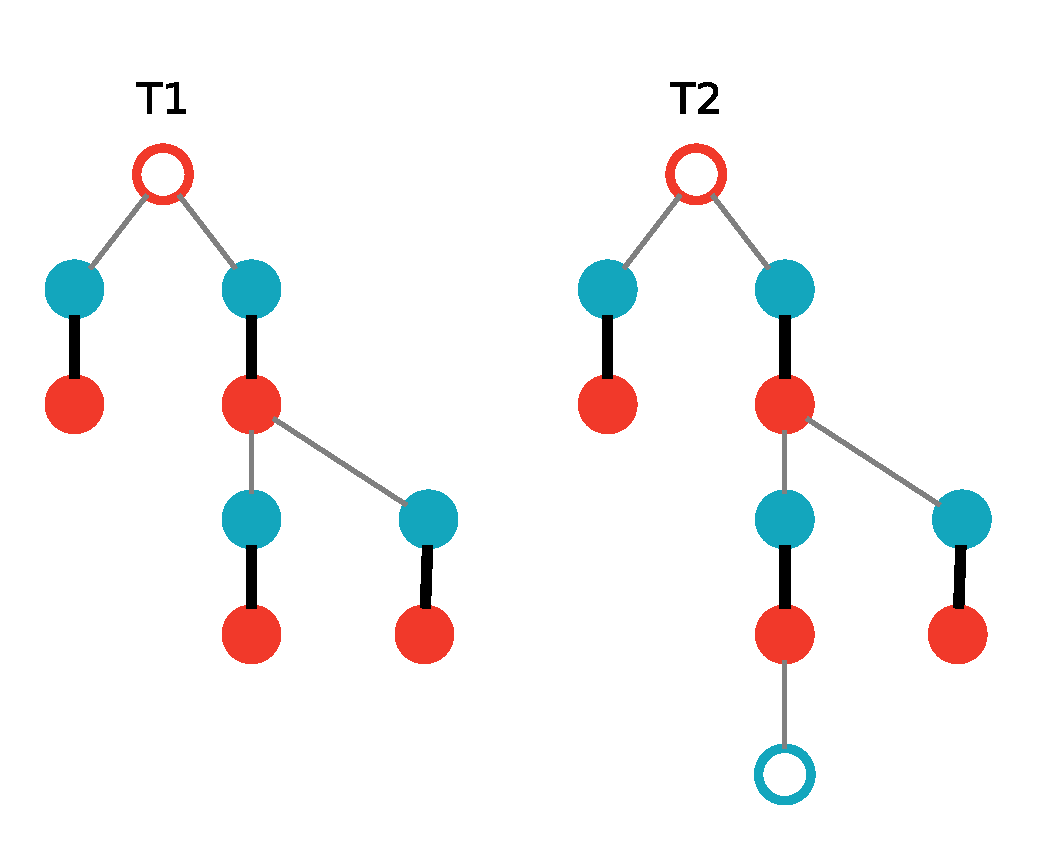
\includegraphics[scale=0.5]{img/trees.eps}
  \caption{M-pokrytý u-strom a M-alternující u-strom.}
  \label{imgTrees}
\end{figure}

%%%%%%%%%%%%%%%%%%%%%%%%%%%%%%%%%%%%%%%%%%%%%%%%%%%%%%%%%%%%%%%%%%%%%%%%%
\section{Sekvenční varianta algoritmu}

\subsection{Datové typy a struktury}

\begin{figure}[ht]
  \centering
  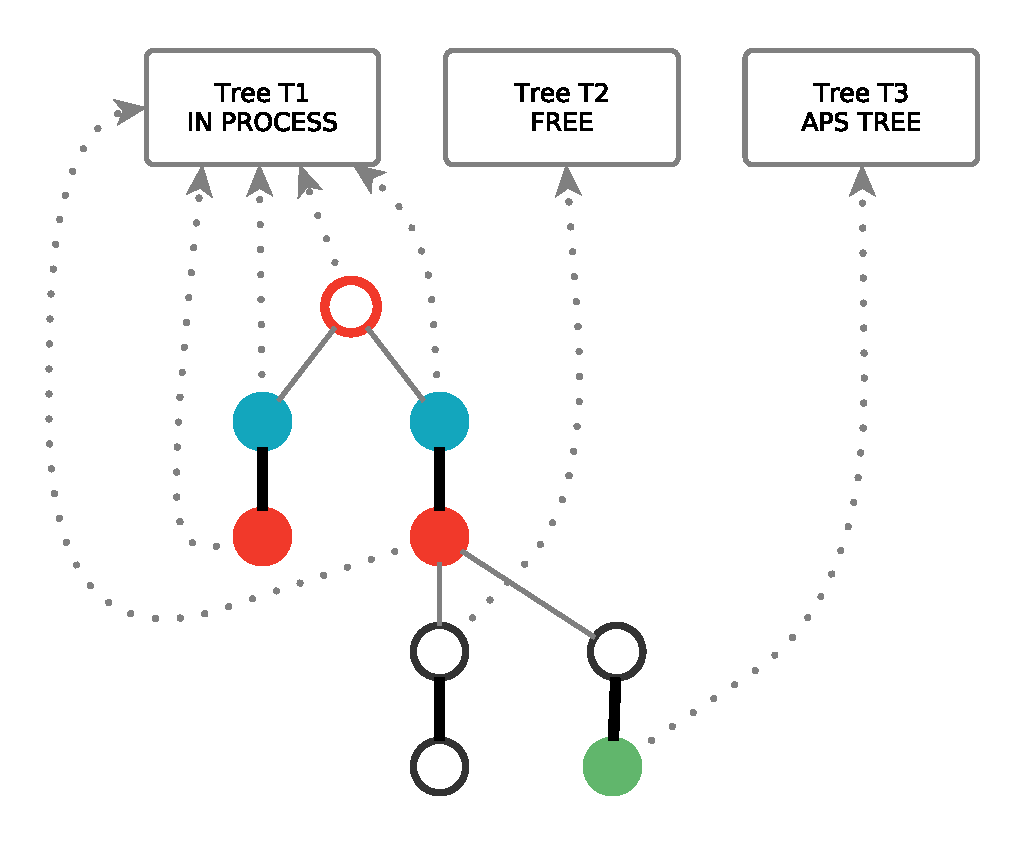
\includegraphics[scale=0.5]{img/implementation.eps}
  \caption{Datové struktury uzlu a stromu.}
  \label{imgStructure}
\end{figure}

\subsection{Popis implementace}


\subsection{Spuštění aplikace}

%%%%%%%%%%%%%%%%%%%%%%%%%%%%%%%%%%%%%%%%%%%%%%%%%%%%%%%%%%%%%%%%%%%%%%%%%
\section{Paralelní varianta algoritmu}

\subsection{Analýza problému}

V popisu Egerváryho algoritmu si lze všimnout, že se vždy pracuje pouze s vytvářeným stromem a jeho nejbližším okolím. Pokud je nalezena $M$-rozšiřující cesta, dochází ke změnám na hranách, které patří do tohoto stromu, pokud je nalezen APS strom, přebarví se pouze uzly tohoto stromu.

Jako přirozený způsob paralelizace Egerváryho algoritmu se nabízí zpracovávání grafu více procesy tak, že každý proces bude vytvářet vlastní strom. Pokud bychom zaručily, že takové stromy budou vždy navzájem disjuktní, s ohledem na předcházející paragraf by paralelní zpracování nijak neovlivnilo fungování Egerváryho algoritmu. Na víceprocesorových počítačích by se však výpočet urychlil.

Disjuktnost stromů ale zaručit nemůžeme, proto je třeba najít způsob, jak se vypořádat s konflikty mezi stromy. Obecná situace je taková, že proces $1$ buduje strom $T_1$, proces $2$ buduje strom $T_2$ a proces $1$ bude chtít k uzlu $v_1$ svého stromu $T_1$ připojit uzel $v_2$ stromu $T_2$. Podle barev uzlů $v_1$ a $v_2$ rozlišujeme následující typy konfliktů.

Konflikt typu B-B je konflikt mezi modrým uzlem $v_1$ a modrým uzlem $v_2$. Příklad takového konfliktu je na obrázku \ref{imgXX}. Na obrázku si můžeme všimnout toho, že v takovém případě existuje $M$-rozšiřující cesta z kořene stromu $T_1$ do kořene stromu $T_2$. Nalezení cesty je žádoucí, proto pokud dojde k takovému konfliktu, lze zastavit růst obou stromů, upravit párování na hranách nalezené cesty a uzly ve stromech přebarvit na bílo, aby byly k dispozici dalším stromům. Konflikt typu R-R pro červené uzly $v_1$, $v_2$ je analogický konfliktu B-B (viz. \ref{imgXX}).

\begin{figure}[ht]
  \centering
  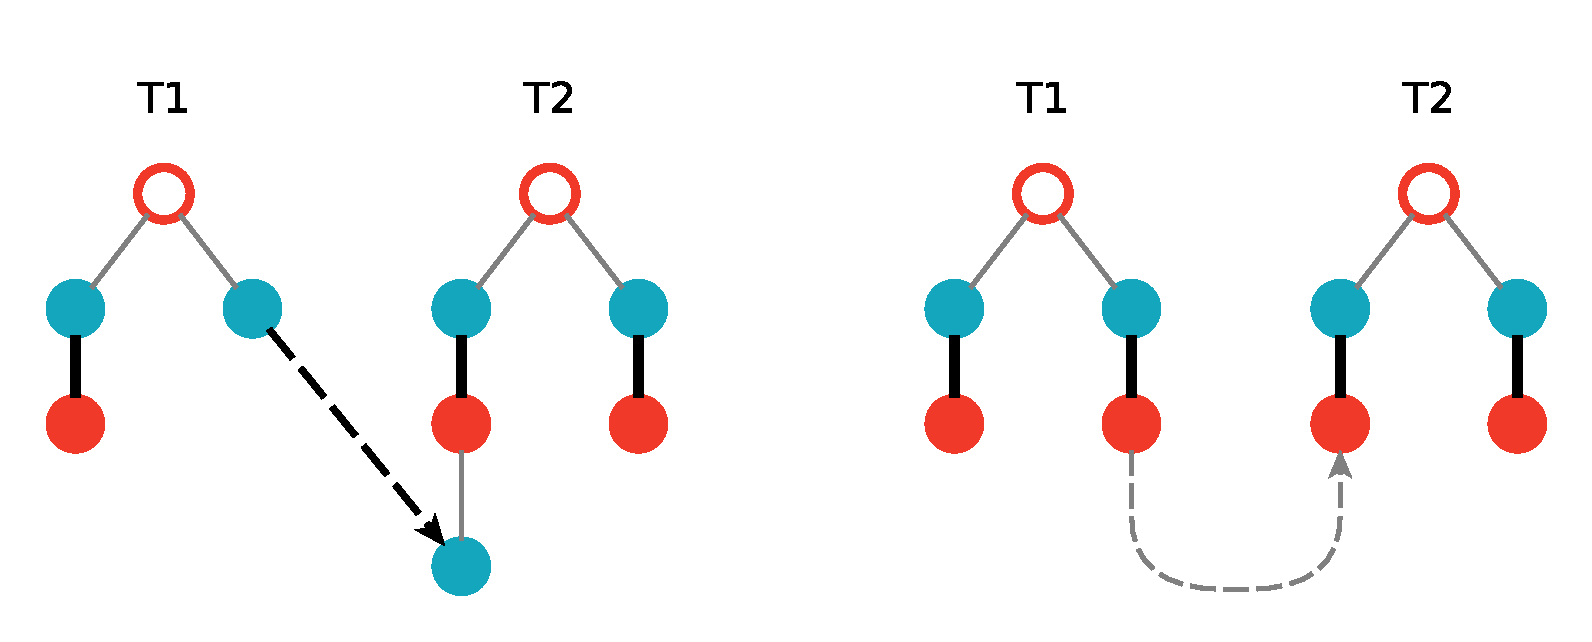
\includegraphics[scale=0.5]{img/XXconflicts.eps}
  \caption{Konflikty B-B a R-R.}
  \label{imgXX}
\end{figure}

Konflikt typu R-B je konflikt mezi červených uzlem $v_1$ a modrým uzlem $v_2$. Na obrázku \ref{imgXY} vidíme, že v tomto případě se $M$-rozšiřující cesta nevytvoří. Nabízí se několik možných řešení. Strom $T_1$ by mohl získat uzel $v_2$, pak by ale strom $T2$ nemohl pokračovat ve výpočtu a všechny jeho uzly by musely být obarveny na bílo a uvolněny. Stejně tak by mohl $T_1$ prohrát uzel $v_2$, $T_2$ by dál pokračoval ve výpočtu a $T_1$ by se ukončil. Třetí možností je ignorace konfliktní hrany. $T_2$ by dál pokračoval ve výpočtu, nijak neovlivněn tímto konfliktem. $T_1$ by taktéž pokračoval ve výpočtu, ale pokud by skončil nalezením APS stromu, tak by své uzly obarvil na bílo a vytvořený strom zahodil.

Konflikt typu B-R je konflikt mezi modrým uzlem $v_1$ a červeným uzlem $v_2$. Z obrázku \ref{imgXY} je patrné, že v takovém případě by z uzlu $v_2$ vedly dvě hrany náležící párování $M$. $M$ by potom nebylo platné párování. Párování může být dočasně neplatné jen v případě, že nějaký strom nalezl $M$-rozšiřující cestu a upravuje párování na hranách této cesty. Pokud jsou oba stromy $T_1$, $T_2$ ve fázi růstu pak párování na hranách vycházejících z uzlů těchto dvou stromů je platné a neměnné. V našem případě předpokládáme, že oba stromy rostou, proto k B-R konfliktu nemůže dojít.

\begin{figure}[ht]
  \centering
  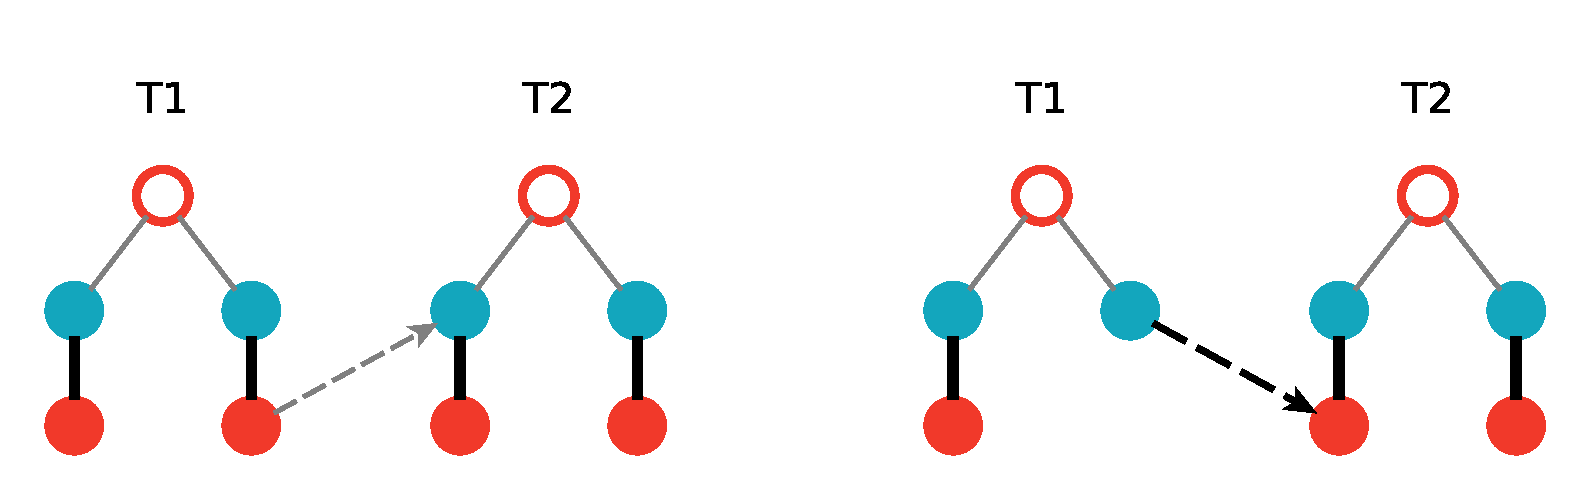
\includegraphics[scale=0.5]{img/XYconflicts.eps}
  \caption{Konflikty R-B a B-R.}
  \label{imgXY}
\end{figure}

Dále je třeba uvažovat o způsobu, jakým se budou synchronizovat procesy. Je zřejmé, že je třeba zaručit, aby s každým uzlem pracoval v jeden okamžik nejvýše jeden proces. Potom bude třeba sychnronizovat přístup ke stromům uzlů. Pokud bychom se inspirovaly návrhem sekvenčního algoritmu, pak informaci o stavu stromu nese pouze strom. Pak při každém přístupu k uzlu je potřeba nejprve zamknout příslušný strom a pak teprve uzel. Pokud očekáváme konflikt, je třeba zamknout oba stromy a konfliktní uzly. Druhou možností je propagovat informaci o stavu stromu do jeho uzlů. Pro přístup k uzlu by pak stačilo zamknutí uzlu.

\subsection{Diskuze k návrhu řešení}

Naše výsledné řešení vyplynulo z několika dalších řešení, která jsme implementovaly a testovaly. 

Konflikt typu R-B jsme původně řešily tak, že proces $1$ vyhrál uzel stromu procesu $2$, pokud jeho strom $T_1$ obsahoval více uzlů než strom $T_2$. Jinak proces $1$ prohrál a byl nucen uvolnit svůj strom. V obou případech došlo k zahození jednoho z konfliktních stromů. Vzhledem k tomu, že další dva typy konfliktů R-R a B-B výpočet urychlují, myslely jsme si, že zpomalení výpočtu konfliktem R-B se ve výsledku neprojeví. Ukázalo se, že to není pravda. K zahazování stromů docházelo neustále a počet vytvořených stromů rostl vzhledem k velikosti vstupního grafu polynomiálně. To značně zpomalovalo výpočet. Efektivnějším řešením konfliktu se ukázala být ignorace konfliktní hrany. Počet vytvořených stromů byl pak lineární a většina $M$-rozšiřujících cest byla nalezena R-R a B-B konflikty.

Synchronizaci procesů jsme zkusily řešit zamykáním stromů. Algoritmus byl tedy velmi podobný sekvenčnímu řešení. Uzly se odkazovaly na stromy a stromy obsahovaly informaci o svém stavu. Rostoucí strom byl ve stavu \texttt{INPROCESS}. Vyvoření APS stromu bylo možné nastavením stavu na \texttt{APSTREE}. Uvolnění stromu proběhlo upravením stavu na \texttt{FREE}. Úprava stavu tak sice byla možná v konstatním čase, ale kdykoliv chtěl proces přidat ke svému stromu nový uzel, musel zamknout svůj strom i strom toho uzlu. Stromy se tak staly úzkým hrdlem programu. To se projevilo zejména tak, že s vyšším počtem dostupných procesorů se časová efektivita programu nezlepšovala.

Řešením tohoto problému byla propagace stavu stromu ze stromu do uzlů. Stav stromu pak bylo možné vyčíst z barvy jeho uzlu. Bílý uzel nepatřil žádnému stromu, zelený uzel patřil APS stromu, modrý a červený uzel patřil zpracovávenému stromu. Toto řešení je výhodné v tom, že pokud chce proces přidat ke svému stromu nový uzel, vyčte z barvy tohoto uzlu, jestli má komunikovat i s jeho stromem, nebo ne. Nevýhodou je časová složitost přebarvení všech uzlů stromu. Důležité však je, že se takto zjednodušila synchronizace, což umožnilo více využívat dostupné procesory.

\subsection{Popis řešení}

Na začátku jsou všechny uzly obarveny na bílo a vloženy do fronty kořenových uzlů. Pokud je kořenová fronta prázdná, proces $i$ se ukončí, jinak z fronty vyzvedne uzel $u$. Pokud je uzel $u$ bilý, proces jej přidá do svého stromu $T_i$ jako kořen a obarví jej na červeno. Proces $i$ začne hledat $M$-rozšiřující cestu. Postupně připojuje k uzlům $v_i$ uzly $v_j$. 

Pokud se pokusí přidat bílý uzel $v_j$, proces uzel obarví na červenou nebo modrou a přivlastní si jej. Pokud se pokusí přidat zelený uzel $v_j$, pak jej ignoruje, neboť uzel patří do APS stromu. Pokud se pokusí přidat červený nebo modrý uzel $v_j$, došlo ke konfliktu. 

\begin{figure}[ht]
  \centering
  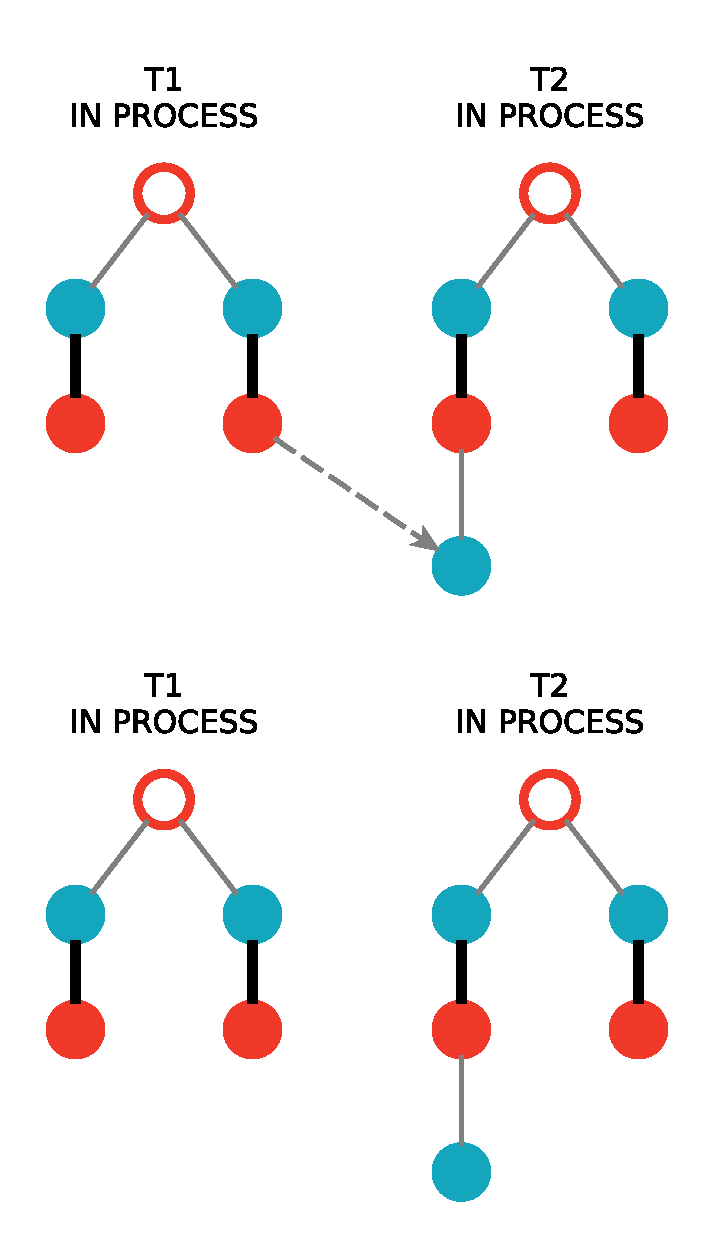
\includegraphics[scale=0.5]{img/inconflict.eps}
  \caption{Řešení R-B konflitu.}
  \label{imgConflict}
\end{figure}

V případě R-B konfliktu proces uzel ignoruje (viz. obrázek \ref{imgConflict}). V případě R-R a B-B konfliktu proces přistoupí ke stromu uzlu. Jestliže je strom $T_j$ ve stavu \texttt{HASPATH}, pak proces uzel ignoruje. Pokud je strom ve stavu \texttt{INPROCESS}, je nalezena $M$-rozšiřující cesta (viz. obrázek \ref{imgHasPath}). Pak proces změní stav stromu $T_j$ na \texttt{HASPATH} a nastaví stromu ukazatel na konec cesty. Následně změní stav svého stromu $T_i$ na \texttt{HASPATH} a nastaví mu ukazatel na konec cesty. Nakonec upraví párování hrany z $v_i$ do $v_j$.

\begin{figure}[ht]
  \centering
  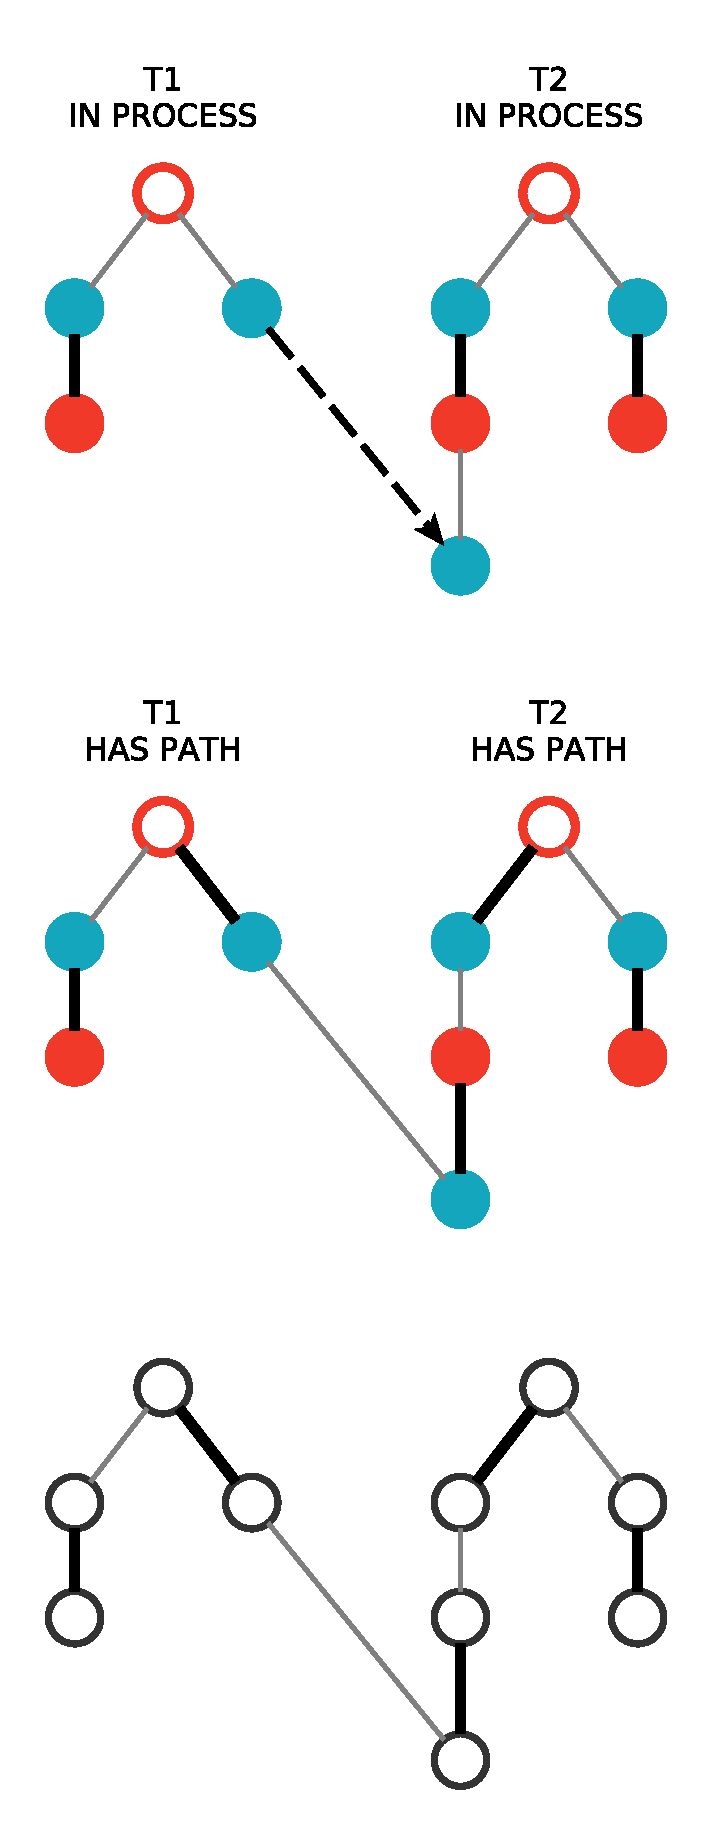
\includegraphics[scale=0.5]{img/haspath.eps}
  \caption{Řešení R-R a B-B konfliktu.}
  \label{imgHasPath}
\end{figure}

Pokud proces $i$ nalezne cestu, nastaví stav stromu $T_i$ na \texttt{HASPATH}. Pokud proces $i$ zjistí, že jeho strom je ve stavu \texttt{HASPATH}, pak upraví párování na nalezené cestě, změní jeho stav na \texttt{FREE} a obarví všechny jeho uzly na bílo. Pokud proces $i$ skončí hledání $M$-rozšiřující cesty nalezením APS stromu a strom $T_i$ nevyvolal žádné R-B konflikty, pak proces nastaví stav stromu na \texttt{APSTREE} a obarví všechny jeho uzly na zeleno. Jestliže strom $T_i$ nějaký R-B konflikt vyvolal, pak proces nastaví jeho stav na \texttt{FREE} a obarví všechny jeho uzly na bílo. Nakonec si proces $i$ vyvedne z fronty kořenových uzlů nový uzel a celý proces se opakuje.

\subsection{Datové typy a struktury}

\subsection{Popis implementace}

\subsection{Spuštění aplikace}

%%%%%%%%%%%%%%%%%%%%%%%%%%%%%%%%%%%%%%%%%%%%%%%%%%%%%%%%%%%%%%%%%%%%%%%%%
\section{Experimenty}

\subsection{Generování vstupních souborů}

Pro vygenerování vstupních souborů jsme v jazyce \texttt{python 2.7} s použitím knihovny \texttt{python-igraph 0.7} napsaly skript \texttt{generator.py}. 
Skript generuje bipartitní neorientované grafy $G=(X,Y,E)$ a ukladá je do souborů \texttt{graph\_x\_y\_p\_m}, kde $x$ je počet uzlů v množině $X$, $y$ je počet uzlů v množině $Y$, $p$ je procentuální vyjádření počtu hran množiny $E$ a $m$ je počet hran v maximálním párování. Pak soubor obsahuje počet uzlů množiny $X \cup Y$, počet hran množiny $E$ a výčet všech dvojic uzlů, mezi kterými existuje v $E$ hrana, přičemž každá hrana je reprezentovaná právě jednou.

Skript je umístěný ve složce \texttt{graph}. Příkazem \texttt{python2.7 generator.py} se podle parametrů nastavených ve scriptu vygeneruje soubor s náhodným grafem. Příkaz \texttt{python2.7 generator.py test} vygeneruje všechny testovací soubory pro naše experimenty. Knihovna \texttt{python-igraph} na školním serveru \texttt{merlin} není dostupná, proto v archivu odevzdáváme část testovacích souborů.



%%%%%%%%%%%%%%%%%%%%%%%%%%%%%%%%%%%%%%%%%%%%%%%%%%%%%%%%%%%%%%%%%%%%%%%%%
\section{Závěr}

%------------------------------------------------------------------------
\begin{thebibliography}{1}
  
  \bibitem{bondy:2008} BONDY, J. A. a U. S. R. MURTY. \emph{Graph theory}. New York: Springer, 2008, xii, 651 s. ISBN 978-1-84628-969-9. 
  
  \bibitem{igraph:2003} \emph{Python-igraph} [online]. \copyright 2003-2013 [cit. 2014-12-13]. Dostupné z: http://igraph.org/python/ 

\end{thebibliography}


%------------------------------------------------------------------------
\end{document}

% end of file
